\documentclass{beamer}
%\usetheme{Warsaw}
%\usetheme{split}
%\usetheme{Amsterdam}
\usetheme{Madrid}
\useoutertheme{miniframes}
\setbeamercovered{invisible}
\setbeamertemplate{navigation symbols}{}
%
\usepackage{tabularx}
\usepackage{graphicx}
\usepackage{algorithm}
\usepackage[noend]{algpseudocode}
% \usepackage{beamerthemesplit}
%
\graphicspath{{../images/}}
%
\title{SSD-based Energy Efficient Cloud Storage}
\author{Salma Rodriguez}
\institute [FIU]{
    Florida International University \\
    %\medskip
    {\emph{srodr063@fiu.edu}}
}
\date{\today}
%
\begin{document}
\begin{frame}
    \titlepage
\end{frame}
%
\section{Introduction}
%
\begin{frame}
    \frametitle{Motivation}
    \begin{block}
	{Solid State Technology}
	High capacity EEPROM devices have been shown to
	reduce energy consumption when used
	as local cache for hard disk drives \cite{key2,key3}.
    \end{block}
    \vspace{7pt}
    \begin{block}
	{Distributed SSD Caching}
	With a distributed caching solution, we hope to increase
	the working set in flash memory and keep server disks spun down.
    \end{block}
    \vspace{7pt}
    \begin{block}
	{Properties to Explore}
	We explore the properties of dynamic spin down of storage
	server disks and replication of cold pages.
    \end{block}
\end{frame}
\begin{frame}
    \frametitle{Linux Device Mapper}
    \begin{tabular}{m{0.465\linewidth}m{0.465\linewidth}}
	%\hline
	\begin{itemize}
	    \item device mapper facilitates mapping between two devices
	    \item only pseudo device in volatile memory visible to applications
	    \item kernel module uses device mapper to map bios sent to pseudo
		device onto real devices (source and target)
	    \item devices may not necessarily be locally attached
	\end{itemize} &
	\begin{figure}
	    %\caption{Device Mapper Layout}
	    \centering 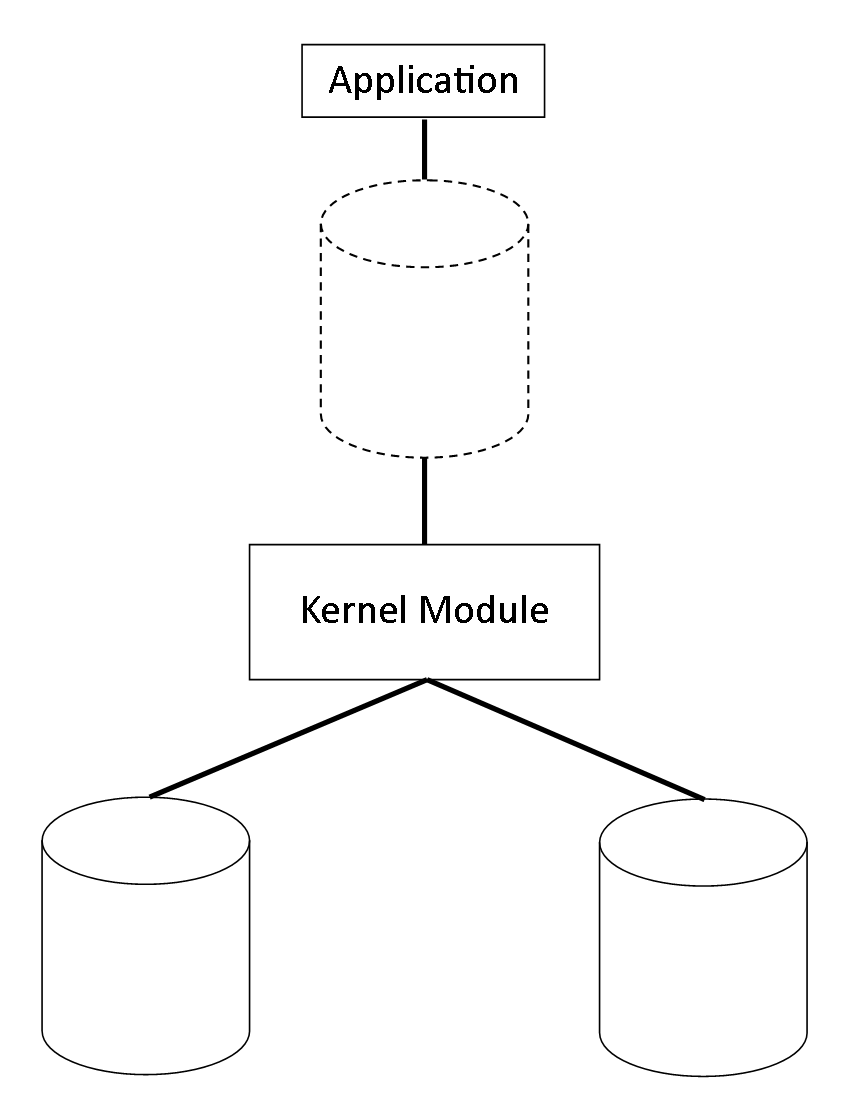
\includegraphics[scale=.23]{DM.png}
	    \label{fig:dm}
	\end{figure} \\
	%\hline
    \end{tabular}
\end{frame}
    \begin{frame}
	\frametitle{Device Mapper Cache}
	\begin{itemize}
	    \item Client machines communicate through iSCSI or AoE network.
	    \item DM Cache takes advantage of spatial and temporal locality
		by storing popular data in a local cache.
	\end{itemize}
	\begin{figure}
	    \centering 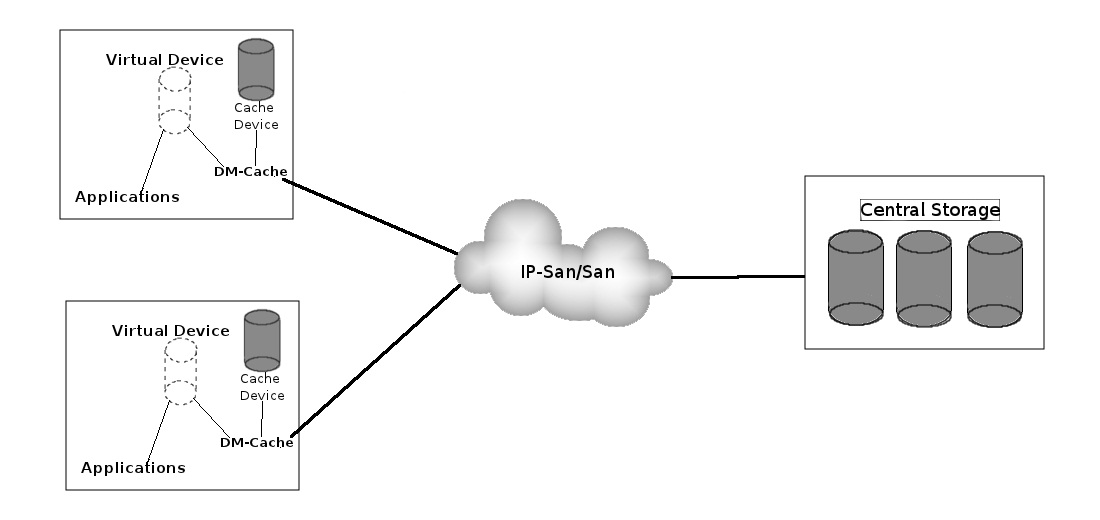
\includegraphics[scale=.30]{DMC.jpg}
	    \label{fig:dmc}
	\end{figure}
    \end{frame}
%
\section{Dynamic Spin Down}
%
\begin{frame}
    \frametitle{Design}
    \begin{figure}
	%\caption{Spinning state is controlled dynamically}
	\bf Figure 1 \rm The state of each disk is controlled dynamically.
	\centering 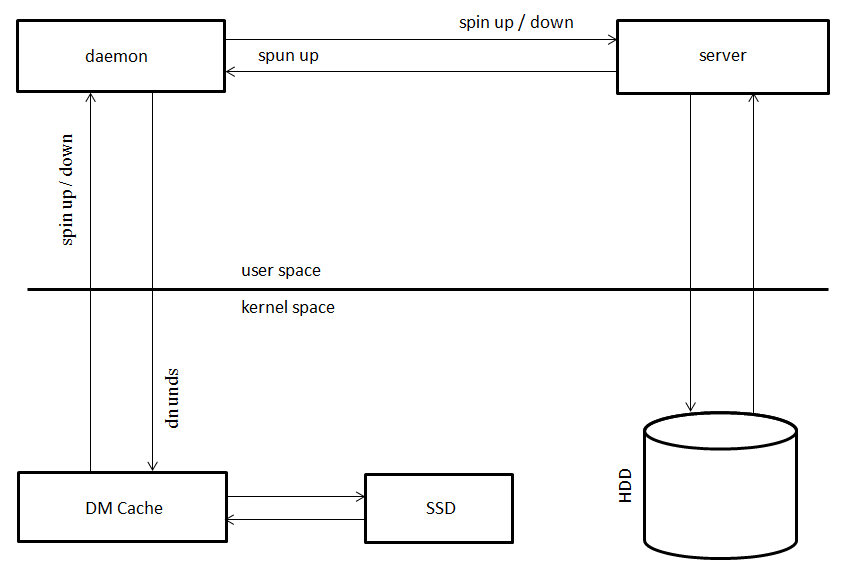
\includegraphics[scale=.43]{drawing.png}
	\label{fig:struct}
    \end{figure}
\end{frame}
\begin{frame}
    \frametitle{Implementation}
    \bf Algorithm 1 \rm spinning the disk up or down dynamically \\
    \algrenewcommand\algorithmicrequire{\textbf{Precondition:}}
    \begin{algorithmic}[1]
	\Require{storage server disk is spinning}
	\Procedure{Spin Up or Down}{}
	\State $T\gets$ constant specified by user
	\While{true}
	    \If{disk is spinning}
		\State $k\gets$ current time in seconds
		\State $c\gets$ time since last cache miss
		\If{$c$ + $T \leq k$}
		    \State spin down the disk and change state to not spinning
		\EndIf
	    \Else \Comment{disk is not spinning}
		\If{DM Cache is blocking on a cache miss}
		    \State spin up the disk and change state to spinning
		    \State unblock DM Cache
		\EndIf
	    \EndIf
	    \State schedule a new process
	\EndWhile
	\EndProcedure
    \end{algorithmic}
\end{frame}
%
\section{Spin Down Results}
%
\begin{frame}
    \frametitle{Spin Down Results}
    \begin{figure}
	\raggedright \bf Figure 2 \rm dynamic disk spin down results for write-intensive workload \\
	The red plot is DM Cache with the spin down daemon. The blue plot
	is iSCSI setup without DM Cache. \\
	\vspace{15pt}
	\centering 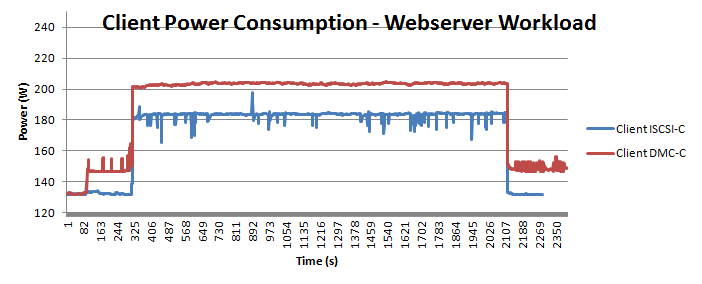
\includegraphics[scale=.45]{image.png}
	\label{fig:results}
    \end{figure}
\end{frame}
\begin{frame}
    \begin{block}{Evaluation}
	\begin{itemize}
	    \item The baseline for our results is a simple iSCSI storage setup.
	    \item We ran a 30 min test using a webserver-based write-intensive workload.
	\end{itemize}
    \end{block}
    \vspace{5pt}
    \begin{block}{Interpretation}
	\begin{itemize}
	    \item DM Cache with the spin down daemon increases power
		by 14 Watt more than the baseline.
	    \item Spin down worker thread performs too many context switches.
	    \item Hypothesis: context switches are a performance
	    	bottleneck and also consume more energy over time.
	    \item Next: use sleep instead of schedule system call.
	\end{itemize}
    \end{block}
\end{frame}
\begin{frame}
    \frametitle{New Spin Down Policy}
    \bf Algorithm 2 \rm new policy using sleep instead of schedule
    \algrenewcommand\algorithmicrequire{\textbf{Precondition:}}
    \begin{algorithmic}[1]
	\Require{storage server disk is spinning}
	\Procedure{Spin Up or Down}{}
	    \State $T\gets$ constant specified by user
	    \While{true}
		\State sleep for $T$ seconds
		\If{disk is spinning}
		    \State $k\gets$ current time in seconds
		    \State $c\gets$ time since last cache miss
		    \If{$c$ + $T \leq k$}
			\State spin down the disk and change state to not spinning
		    \EndIf
		\Else \Comment{disk is not spinning}
		    \If{DM Cache is blocking on a cache miss}
			\State spin up the disk and change state to spinning
			\State unblock DM Cache
		    \EndIf
		\EndIf
	    \EndWhile
	\EndProcedure
    \end{algorithmic}
\end{frame}

\section{Future Work}
%
\begin{frame}
    \frametitle{Cooperative Caching}
    \begin{block}{Basic Idea}
	\begin{itemize}
	    \item Save power by sending unused clean data to neighboring caches
		instead of evicting from the cache to the storage server.
	    \item Assumption: not all clients will have their cache full to capacity.
	    \item Tradeoff between free space and caching fairness:
	    \vspace{5pt}
	    \center{
		$\textrm{benefit} = \frac{\textrm{free space}}
		{\textrm{space taken by other caches}}$
	    }
	\end{itemize}
    \end{block}
    \begin{block}{Challenges}
	\begin{itemize}
	    \item Choose efficient cache replacement policy to
		send pages that are less popular to other caches.
	    \item Cache cooperatively and handle nodes as they dynamically
		join and exit the network of peer caches.
	\end{itemize}
    \end{block}
\end{frame}
%begin{frame}
%       \frametitle{Consistent Hashing}
%       Idea: may save power by caching data with as little disruption
%       as possible when nodes join and exit the network. \\
%       \begin{theorem}
%       	For any set of N nodes and K keys, with high probability:
%       	\begin{enumerate}
%       		\item Each node is responsible for at most (1 + $\epsilon$)K/N keys.
%       		\item When an (N + 1)st node joins or leaves the network,
%       		responsibility for O(K/N) keys changes to the joining node, or from
%       		the leaving node.
%       	\end{enumerate}
%       \end{theorem}
%       Here $\epsilon$ may vary but has an upper bound of \textit{O(log N)} \cite{key1}.
%       \begin{block}
%       	{Challenge}
%       	Dynamically copy data and maintain mapping of block addresses to network nodes
%       	as data is propagated to the cache of neighboring clients.
%       \end{block}
%end{frame}
%
\section{References}
%
\begin{frame}
    \frametitle{References}
    \footnotesize {
	\begin{thebibliography}{98}
	    \bibitem[1]{key1} I. Stoica, R. Morris, D. Karger, M. F. Kaashoek, and H. Balakrishnan.
		Chord: A Scalable Peer-to-peer Lookup Service for Internet Applications.
		\emph{Special Interest Group on Data Communication (SIGCOMM '01)},
		San Diego, California, Aug. 2001.
	    \bibitem[2]{key2} J.D. Garcia, J. Carretero, and F. Garcia.
		Saving power in flash and disk hybrid storage system.
		\emph{Modeling, Analysis \& Simulation of Computer and Telecommunication Systems
	    (MASCOTS 2009)}, London, U.K., Sep. 2009.
	\bibitem[3]{key3} T. Bisson and S. A. Brandt.
	    Reducing Energy Consumption with a Non-Volatile Storage Cache.
	    \emph{International Workshop on Software Support for Portable Storage (IWSSPS)
		held in conjunction with the IEEE Real-Time and Embedded Systems and Applications
	    Symposium (RTAS 2005)}, Mar. 2005.
	\end{thebibliography}
    % \bf Acknowledgements \rm I extend my gratitude to Jorge Cabrera for assisting me with the shell
	%scripts that allow the spin down daemon to interact with the disks on the storage server. I
	%am also thankful to Jesus Ramos for pointing out the "grammar squiggles" in my draft of
	%figure 1 (mental note: don't use Microsoft Word for drawing figures).
    }
\end{frame}
%
\end{document}
